\chapter{Mathematical Review}

The review of set theory contained herein adopts a naive point of view.
We assume that the meaning of a set as a collection of objects is intuitively clear.
A rigorous analysis of this concept belongs to the foundations of mathematics and mathematical logic.
Although we shall not initiate a study of these fields, the rules we follow in dealing with sets are derived from them.
A \emph{set} is a collection of objects, which are the \emph{elements} of the set. \index{Set} \index{Element}

\begin{center}
\begin{psfrags}
\psfrag{1}[c]{$1$}
\psfrag{2}[c]{$2$}
\psfrag{3}[c]{$3$}
\psfrag{4}[c]{$4$}
\psfrag{5}[c]{$5$}
\psfrag{6}[c]{$6$}
\psfrag{7}[c]{$7$}
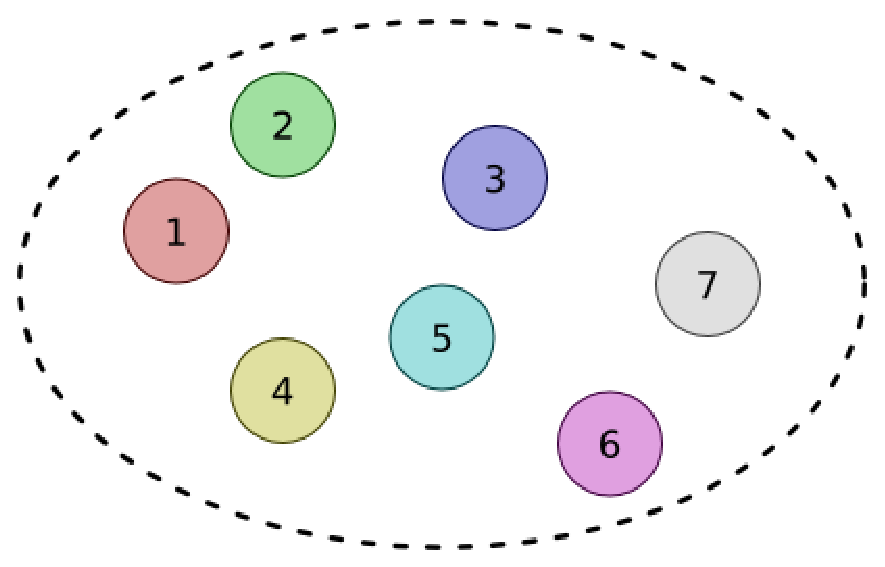
\includegraphics[height=3.825cm]{Figures/1Chapter/basicset}
\end{psfrags}
\end{center}

If an element $x$ belongs to a set $S$, we express this fact by writing $x \in S$.
If $x$ does not belong to $S$, we write $x \notin S$.
We use the equality symbol to denote \emph{logical identity}.
For instance, $x = y$ means that $x$ and $y$ are symbols denoting the same object.
Similarly, the equation $S = T$ states that $S$ and $T$ are two symbols for the same set.
In particular, the sets $S$ and $T$ contain precisely the same elements.
If $x$ and $y$ are different objects then we write $x \neq y$.
Also, we can express the fact that $S$ and $T$ are different sets by writing $S \neq T$.

A set $S$ is a \emph{subset} of $T$ if every element of $S$ is also contained in $T$. \index{Subset}
We express this relation by writing $S \subset T$.
Note that this definition does not require $S$ to be different from $T$.
In fact, $S = T$ if and only if $S \subset T$ and $T \subset S$.
If $S \subset T$ and $S$ is different from $T$, then $S$ is a \emph{proper subset} of $T$ and we write $S \subsetneq T$. \index{Proper subset}

There are many ways to specify a set.
If the set contains only a few elements, one can simply list the objects in the set;
\begin{equation*}
S = \{ x_1, x_2, x_3 \} .
\end{equation*}
The content of a set can also be enumerated whenever $S$ has a countable number of elements,
\begin{equation*}
S = \{ x_1, x_2, \ldots \} .
\end{equation*}
Usually, the way to specify a set is to take some collection $S$ of objects and some property that elements of $S$ may or may not possess, and to form the set consisting of all elements of $S$ having that property.
For example, starting with the integers $\Integers$, we can form the subset of $S$ consisting of all even numbers,
\begin{equation*}
S = \{ x \in \Integers | x \text{ is an even number} \}.
\end{equation*}
More generally, we denote the set of all elements that satisfy a certain property $P$ by
\begin{equation*}
S = \{ x | x \text{ satisfies } P \} .
\end{equation*}
The braces are to be read as the words ``the set of'' whereas the symbol $|$ stands for the words ``such that.''

It is convenient to introduce two special sets.
The \emph{empty set}, denoted by $\emptyset$, is a set that contains no elements. \index{Empty set}
The \emph{universal set} is the collection of all objects of interest in a particular context, and it is denoted by $\Omega$.
Once a universal set $\Omega$ is specified, we need only consider sets that are subsets of $\Omega$.
In the context of probability, $\Omega$ is often called the \emph{sample space}. \index{Sample space}

The \emph{complement} of a set $S$, with respect to the universal set $\Omega$, is the collection of all objects in $\Omega$ that do not belong to $S$, \index{Complement}
$S^{\Complement} = \{ x \in \Omega | x \notin S \}$.
We note that $\Omega^{\Complement} = \emptyset$.


\section{Elementary Set Operations}

Probability theory makes extensive use of elementary set operations.
Below, we review the ideas of set theory, and establish basic terminology and notation.
Consider two sets, $S$ and $T$.

\begin{center}
\begin{psfrags}
\psfrag{S}[c]{$S$}
\psfrag{T}[c]{$T$}
\includegraphics[height=3.03cm]{Figures/1Chapter/sets}
\end{psfrags}
\end{center}

The \emph{union} of sets $S$ and $T$ is the collection of all elements that belong to $S$ or $T$ (or both), and it is denoted by $S \cup T$. \index{Union}
Formally, we define the union of these two sets by
\begin{equation*}
S \cup T = \{ x | x \in S \text{ or } x \in T \} .
\end{equation*}

\begin{center}
\begin{psfrags}
\psfrag{U}[c]{$S \cup T$}

\includegraphics[height=3.03cm]{Figures/1Chapter/union}
\end{psfrags}
\end{center}

The \emph{intersection} of sets $S$ and $T$ is the collection of all elements that belong to $S$ and $T$. \index{Intersection}
It is denoted by $S \cap T$, and it can be expressed mathematically as
\begin{equation*}
S \cap T = \{ x | x \in S \text{ and } x \in T \} .
\end{equation*}

\begin{center}
\begin{psfrags}
\psfrag{I}[c]{$S \cap T$}
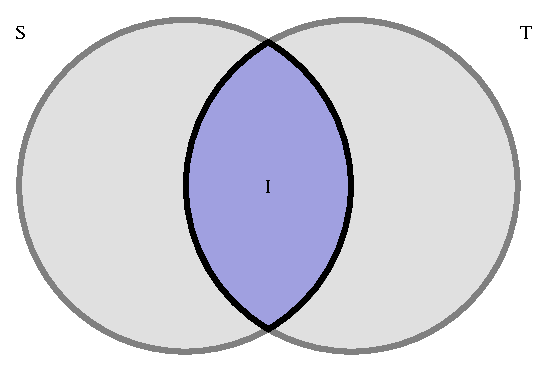
\includegraphics[height=3.03cm]{Figures/1Chapter/intersection}
\end{psfrags}
\end{center}

When $S$ and $T$ have no elements in common, we write $S \cap T = \emptyset$.
We also express this fact by saying that $S$ and $T$ are \emph{disjoint}. \index{Disjoint sets}
More generally, a collection of sets is said to be disjoint if no two sets have a common element.
A collection of sets is said to form a \emph{partition} of $S$ if the sets in the collection are disjoint and their union is $S$. \index{Partition}

\begin{center}
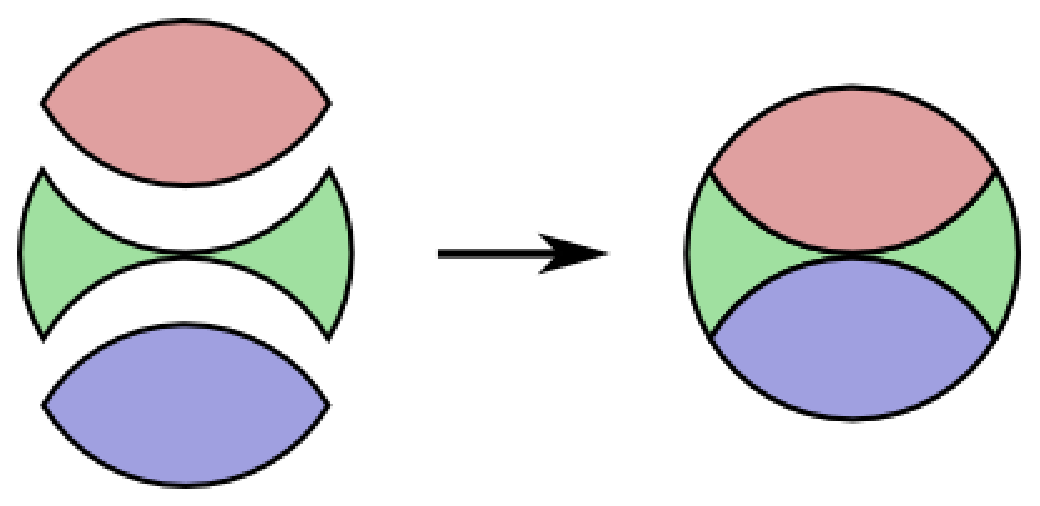
\includegraphics[height=4.23cm]{Figures/1Chapter/setpartition}
\end{center}

The \emph{difference} of two sets, denoted by $S - T$, is defined as the set consisting of those elements of $S$ that are not in $T$,
\begin{equation*}
S - T = \{ x | x \in S \text{ and } x \notin T \} .
\end{equation*}
This set is sometimes called the complement of $T$ relative to $S$, or the complement of $T$ in $S$.

\begin{center}
\begin{psfrags}
\psfrag{D}[c]{$S - T$}
\includegraphics[height=3.03cm]{Figures/1Chapter/difference}
\end{psfrags}
\end{center}

We have already looked at the definition of the union and the intersection of two sets.
We can also form the union or the intersection of arbitrarily many sets.
This is defined in the obvious way,
\begin{align*}
\bigcup_{\alpha \in \IndexSet} S_{\alpha}
&= \{ x | x \in S_{\alpha} \text{ for some } \alpha \in \IndexSet \} \\
\bigcap_{\alpha \in \IndexSet} S_{\alpha}
&= \{ x | x \in S_{\alpha} \text{ for all } \alpha \in \IndexSet \} .
\end{align*}
The index set $\IndexSet$ can be finite or even infinite.


\section{Additional Rules and Properties}

Given a collection of sets, it is possible to form new ones by applying elementary set operations to them.
As in algebra, one uses parentheses to indicate precedence.
For instance, $R \cup (S \cap T)$ denotes the union of two sets $R$ and $S \cap T$, while $(R \cup S) \cap T$ represents the intersection of two sets $R \cup S$ and $T$.
The sets thus formed are quite different.

\begin{center}
\begin{psfrags}
\psfrag{P1}[c]{$R \cup (S \cap T)$}
\psfrag{P2}[c]{$(R \cup S) \cap T$}
\includegraphics[height=4.53cm]{Figures/1Chapter/triple}
\end{psfrags}
\end{center}

Sometimes different combinations of operations lead to the same set.
For instance, we have the two distributive laws
\begin{align*}
R \cap (S \cup T) &= (R \cap S) \cup (R \cap T) \\
R \cup (S \cap T) &= (R \cup S) \cap (R \cup T).
\end{align*}
Two particularly useful equivalent combinations of operations are given by \emph{De~Morgan's laws}, which state that \index{De Morgan's laws}
\begin{align*}
R - (S \cup T) &= (R - S) \cap (R - T) \\
R - (S \cap T) &= (R - S) \cup (R - T).
\end{align*}
These two laws can be generalized to
\begin{align*}
\left( \bigcup_{\alpha \in \IndexSet} S_{\alpha} \right)^{\Complement}
&= \bigcap_{\alpha \in \IndexSet} S_{\alpha}^{\Complement} \\
\left( \bigcap_{\alpha \in \IndexSet} S_{\alpha} \right)^{\Complement}
&= \bigcup_{\alpha \in \IndexSet} S_{\alpha}^{\Complement}
\end{align*}
when multiple sets are involved.
To establish the first equality, suppose that $x$ belongs to $\left( \bigcup_{\alpha \in \IndexSet} S_{\alpha} \right)^{\Complement}$.
Then $x$ is not contained in $\bigcup_{\alpha \in \IndexSet} S_{\alpha}$.
That is, $x$ is not an element of $S_{\alpha}$ for any $\alpha \in \IndexSet$.
This implies that $x$ belongs to $S_{\alpha}^{\Complement}$ for all $\alpha \in \IndexSet$, and therefore $x \in \bigcap_{\alpha \in \IndexSet} S_{\alpha}^{\Complement}$.
We have shown that $\left( \bigcup_{\alpha \in \IndexSet} S_{\alpha} \right)^{\Complement} \subset \bigcap_{\alpha \in \IndexSet} S_{\alpha}^{\Complement}$.
The converse inclusion is obtained by reversing the above argument.
The second law can be obtained in a similar fashion.


\section{Cartesian Products}

There is yet another way to create new sets form existing ones.
It involves the notion of an \emph{ordered pair} of objects. \index{Ordered pair}
Given sets $S$ and $T$, the \emph{cartesian product} $S \times T$ is the set of all ordered pairs $(x, y)$ for which $x$ is an element of $S$ and $y$ is an element of $T$, \index{Cartesian product}
\begin{equation*}
S \times T = \{ (x, y) | x \in S \text{ and } y \in T \} .
\end{equation*}

\begin{center}
\begin{psfrags}
\psfrag{1}[c]{$1$}
\psfrag{2}[c]{$2$}
\psfrag{3}[c]{$3$}
\psfrag{a}[c]{$a$}
\psfrag{b}[c]{$b$}
\includegraphics[height=3.06cm]{Figures/1Chapter/cartesianproduct}
\end{psfrags}
\end{center}


\section{Set Theory and Probability}

Set theory provides a rigorous foundation for modern probability and its axiomatic basis.
It is employed to describe the laws of probability, give meaning to their implications and answer practical questions.
Being familiar with basic definitions and set operations is key in understanding the subtleties of probability; it helps overcome its many challenges.
A working knowledge of set theory becomes critical when modeling measured quantities and evolving processes that appear random, a invaluable skill for engineers.

